\section{Channel System}
\label{sec:channelSystem}

To justify our choice of a typed-parameterized extension of a channel system, we need to establish our requirements. Recalling our motivation example (Section \ref{sec:motivation}), the team's members execute tasks in parallel and each member exchange information with the leader, changing its decisions based on the instructions its receives, i.e, which tasks are allocated for it. Moreover, dynamic events also changes its attitudes, e.g, sensor failure causes an information exchange with the leader, to update task's allocation process. Thus, the capability of coping context changes eventually arising during a mission in a \textit{nondeterministic} way motivate the use of \textit{program graphs}~\cite{modelcheckingBaier}. Furthermore, the execution of parallel processes and the communication among members are requirements that prompt the use of \textit{channel systems}~\cite{modelcheckingBaier}.

A channel system is composed of a group of data-dependent processes communicating with each via \textit{communication actions}~\cite{modelcheckingBaier}. With a program graph representing each process, transitions among states can be classified between conditional transitions or communication actions. Conditional transitions are important to avoid transitioning to states undesirably, according to boolean evaluation~\cite{modelcheckingBaier} defined during planning. The last type of transition works transmitting values through channels or receiving values from channels and assigning them to variables~\cite{modelcheckingBaier}. Additionally, channels can have a finite or infinite capacity of messages in a single channel, as well as a specified type of messages that can be stored in it. Finally, channel systems provide a notion of synchronization, whereas channels with a capacity different from zero function in a \textit{asynchronous} way and null capacity channels represent \textit{synchronous} communication~\cite{modelcheckingBaier}.

\begin{figure}[!ht]
    \centering
    \scalebox{.75}{

\tikzset{every picture/.style={line width=0.75pt}} %set default line width to 0.75pt        

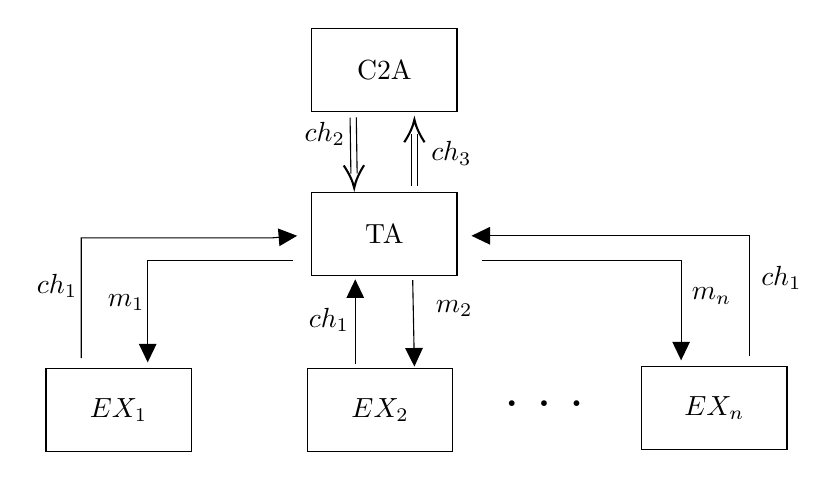
\begin{tikzpicture}[x=0.75pt,y=0.75pt,yscale=-1,xscale=1]
%uncomment if require: \path (0,225); %set diagram left start at 0, and has height of 225

%Shape: Rectangle [id:dp7793135649662085] 
\draw   (146,89) -- (216,89) -- (216,129) -- (146,129) -- cycle ;
%Shape: Rectangle [id:dp8388066725390221] 
\draw   (146,10) -- (216,10) -- (216,50) -- (146,50) -- cycle ;
%Shape: Rectangle [id:dp48691256180587716] 
\draw   (18,174) -- (88,174) -- (88,214) -- (18,214) -- cycle ;
%Straight Lines [id:da7136052167478543] 
\draw    (194.67,131.33) -- (195.44,170) ;
\draw [shift={(195.5,173)}, rotate = 268.85] [fill={rgb, 255:red, 0; green, 0; blue, 0 }  ][line width=0.08]  [draw opacity=0] (8.93,-4.29) -- (0,0) -- (8.93,4.29) -- cycle    ;
%Straight Lines [id:da1199439366931846] 
\draw    (35,169) -- (35,111) -- (127,111) -- (136.01,110.25) ;
\draw [shift={(139,110)}, rotate = 535.24] [fill={rgb, 255:red, 0; green, 0; blue, 0 }  ][line width=0.08]  [draw opacity=0] (8.93,-4.29) -- (0,0) -- (8.93,4.29) -- cycle    ;
%Shape: Rectangle [id:dp8070909053866772] 
\draw   (305,173) -- (375,173) -- (375,213) -- (305,213) -- cycle ;
%Shape: Rectangle [id:dp18131918632628874] 
\draw   (144,174) -- (214,174) -- (214,214) -- (144,214) -- cycle ;
%Straight Lines [id:da23459308482895536] 
\draw    (357,168) -- (357,110) -- (226,110) ;
\draw [shift={(223,110)}, rotate = 360] [fill={rgb, 255:red, 0; green, 0; blue, 0 }  ][line width=0.08]  [draw opacity=0] (8.93,-4.29) -- (0,0) -- (8.93,4.29) -- cycle    ;
%Straight Lines [id:da9340034396500284] 
\draw    (228,122) -- (324,122) -- (324,167) ;
\draw [shift={(324,170)}, rotate = 270] [fill={rgb, 255:red, 0; green, 0; blue, 0 }  ][line width=0.08]  [draw opacity=0] (8.93,-4.29) -- (0,0) -- (8.93,4.29) -- cycle    ;
%Straight Lines [id:da26523318096149495] 
\draw    (137,122) -- (67,122) -- (67,168) ;
\draw [shift={(67,171)}, rotate = 270] [fill={rgb, 255:red, 0; green, 0; blue, 0 }  ][line width=0.08]  [draw opacity=0] (8.93,-4.29) -- (0,0) -- (8.93,4.29) -- cycle    ;
%Straight Lines [id:da6224238934860249] 
\draw    (167,172) -- (167,134) ;
\draw [shift={(167,131)}, rotate = 450] [fill={rgb, 255:red, 0; green, 0; blue, 0 }  ][line width=0.08]  [draw opacity=0] (8.93,-4.29) -- (0,0) -- (8.93,4.29) -- cycle    ;
%Straight Lines [id:da30878293142018354] 
\draw    (167.5,52.98) -- (167.9,79.98)(164.5,53.02) -- (164.9,80.02) ;
\draw [shift={(166.5,87)}, rotate = 269.15999999999997] [color={rgb, 255:red, 0; green, 0; blue, 0 }  ][line width=0.75]    (10.93,-4.9) .. controls (6.95,-2.3) and (3.31,-0.67) .. (0,0) .. controls (3.31,0.67) and (6.95,2.3) .. (10.93,4.9)   ;
%Straight Lines [id:da1036410124215259] 
\draw    (197,61) -- (197,86)(194,61) -- (194,86) ;
\draw [shift={(195.5,54)}, rotate = 90] [color={rgb, 255:red, 0; green, 0; blue, 0 }  ][line width=0.75]    (10.93,-4.9) .. controls (6.95,-2.3) and (3.31,-0.67) .. (0,0) .. controls (3.31,0.67) and (6.95,2.3) .. (10.93,4.9)   ;

% Text Node
\draw (181,30) node   [align=left] {C2A};
% Text Node
\draw (181,109) node   [align=left] {TA};
% Text Node
\draw (53,194) node    {$EX_{1}$};
% Text Node
\draw (23.33,134.33) node    {$ch_{1}$};
% Text Node
\draw (214.67,145) node    {$m_{2}$};
% Text Node
\draw (340,193) node    {$EX_{n}$};
% Text Node
\draw (179,194) node    {$EX_{2}$};
% Text Node
\draw (258,191) node  [font=\Large] [align=left] {\textbf{. . .}};
% Text Node
\draw (338.67,139) node    {$m_{n}$};
% Text Node
\draw (56.67,142) node    {$m_{1}$};
% Text Node
\draw (154.33,150.33) node    {$ch_{1}$};
% Text Node
\draw (372.33,130.33) node    {$ch_{1}$};
% Text Node
\draw (152.33,60.83) node    {$ch_{2}$};
% Text Node
\draw (213.33,70.33) node    {$ch_{3}$};


\end{tikzpicture}}
    \caption{Channel System Representation}
    \label{fig:CS}
\end{figure}

Figure \ref{fig:CS} illustrates our channel system. The proposed channel system describe our coordination strategy. We decided to model our coordination using separate roles, mainly due to its nature of isolating functional aspects~\cite{roleOrientedModeling}. Also, roles are used to define positions within an organization, encapsulating certain tasks, responsibilities, and goals that an owner of a role has to fulfil~\cite{roleOrientedModeling}. Thus, each member of the team can posses program graphs that describe each role, and more than one role can coexist in the same entity. Also, during maneuvering between different C2 approaches~\cite{france2014}, roles can be added or removed, providing more possibilities to the team during the mission.

To separate roles, each one with a proper and unique set of functions, we divided the coordination aspect among two different roles:

\begin{itemize}
    \item Executor: responsible for executing tasks and providing feedback about which tasks it did to the member with the task allocator role.
    \item Task Allocator: responsible for distributing tasks throughout the team, allocating tasks within the knowledge of member's attributes, such as fuel, sensors, etc.
    \item C2 Approach Selector: responsible for detecting potential sufficient approaches, due to some drop in performance reported by task allocator.
\end{itemize}

Furthermore, each member execute its role or set of roles encapsulated in it. For instance, as depicted in Figure \ref{fig:CS}, each member who detains an executor role communicates with the leader, i.e, member who holds the role task allocator, using channel \textit{$ch_1$} in a asynchronous manner. In a similar way, the leader provides tasks to each executor member using channel \textit{$m_2$}. Finally, the C2 approach selector role and task allocator role exchange information using synchronized channels \textit{$ch_2$} and \textit{$ch_3$} to asses performance and check if a maneuver is crucial to maintain quality of execution during the mission. These last channels use synchronized communication because the task allocator role provides performance information using channel \textit{$ch_3$} and waits for the C2 approach selector's response to know if a maneuver might happen. Until this feedback information approaches the channel \textit{$ch_2$}, the task allocator role stops allocating tasks to the remaining members. However, members that execute tasks, i.e, possess executor roles, and allocate tasks, i.e, holds task allocator role, don't need to wait for any response and can continue executing tasks or allocating tasks, justifying the asynchronous communication between these roles.